\documentclass[output=paper]{langsci/langscibook} 
\ChapterDOI{10.5281/zenodo.3975803}
\author{Henrik Liljegren \affiliation{University of Stockholm}} 

\title{Emerging epistemic marking in Indo-Aryan Palula}
%\shorttitlerunninghead{}

% \title{\texorpdfstring{Word formation and word history:\\ The case of
%  \textsc{capitalist} and \textsc{capitalism}}{Word formation and word
% history:  CAPITALIST and
% CAPITALISM}}

% \renewcommand{\lsCollectionPaperFooterTitle}{Emerging epistemic marking in Indo-Aryan Palula}

 

\abstract{While evidentiality is neither systematically nor obligatorily signaled in Indo-Aryan Palula [phl; phal1254] (Pakistan), it can be observed in so-called scattered coding. It is most obviously reflected in three sub-systems of the language: a) as a secondary effect of tense—aspect differentiation, mostly clearly seen in the use of the perfect for indirect evidence vis-à-vis the use of the simple past for direct evidence; b) by a set of utterance-final mood markers, involving an emerging three-way paradigmatic contrast: \textit{thaní} as quotative, \textit{maní} as hearsay and \textit{ɡa} as inferred knowledge; and c) by (at least) one member of a set of second-position discourse particles, \textit{xu}, marking surprise. Although evidentiality contrasts akin to the perfect vs. simple past were indeed part of the ancestral Indo-Aryan tense system, there are plenty of parallels in adjacent languages to the epistemic contrasts noted for Palula, suggesting that more recent language contact must have contributed to, or largely facilitated, the emergence of epistemic marking in the language.}

\begin{document}
\maketitle

\section{Introduction} 

While evidentiality, mirativity and related notions have been discussed at length for Sino-Tibetan (\citealt{DeLancey1986}; \citeyear{DeLancey2001}) and for Turkic languages (\citealt{Johanson2000}; \citeyear{Johanson2003}), relatively little attention has been given to similar phenomena in the multilingual Hindukush-Karakoram (Afghanistan, Pakistan, Kashmir), a mountainous region home to approximately 50 distinct – mostly Indo-Iranian – languages, lying at the crossroads of South Asia and the Tibetan and the Turkic worlds. Only some preliminary suggestions regarding evidentiality and its origin in the region have been offered, and a few language-specific studies focussing on epistemic aspects have been carried out (see \sectref{s:hl2}). While in a few languages, contrasts in the realm of evidentiality are actually part of verbal morphology, in others it is mainly indicated with particles, or else such distinctions are present in “scattered coding”, i.e. not as part of a single sub-system but instead encoded in various parts of the grammar. In the present study, texts belonging to a corpus resulting from recent fieldwork on Indo-Aryan Palula have been analysed, and some preliminary conclusions as well as open-ended questions are offered regarding various types of epistemic marking found in the language, their possible semantic scope and their relationship to other language-particular grammatical distinctions. It has been found that epistemic marking is entailed in some tense-aspect distinctions (\sectref{s:hl3}); in the use of mood-markers (\sectref{s:hl4}); and in the use of discourse particles (\sectref{s:hl5}). In as much detail as possible, derivational paths will be discussed (see \sectref{s:hl6}), and also language-contact effects, e.g. the possible influence of grammaticalized inferentiality in neighbouring languages or in languages of wider communication on Palula. The findings of the study are summarized in \sectref{s:hl7}.

\section{Background}\label{s:hl2}

Palula [iso 639-3: phl; glottocode: phal1254] is an Indo-Aryan language belonging to the Shina group. It is spoken by approximately 10,000 people in the southern part of Chitral district in northern Pakistan (35.38, 71.78; see \figref{fig:hl1}). Speakers are to a varying degree bilingual in Khowar, another Indo-Aryan language widely spoken in Chitral, and/or in Pashto, an Iranian language that is one of the most important lingua francas of northwestern Pakistan. Educated speakers also know Urdu, the nation-wide lingua franca of Pakistan, and to a lesser extent English. The author conducted linguistic fieldwork in this language, primarily in the period 1998 to 2006, with the compilation of a corpus of Palula narratives and other texts as one of its aims.\footnote{The interested reader is encouraged to consult the following works dedicated to the description and documentation of Palula: phonetics and phonology (\citealt{LiljegrenHaider2009}); morphology and syntax (\citealt{Liljegren2010}; \citeyear{Liljegren2016}); vocabulary and semantics (\citealt{LiljegrenHaider2011}; \citeyear{LiljegrenHaider2015a}); glossed and translated texts (\citealt{LiljegrenHaider2015b}).}
In the present study, that corpus has been consulted, along with various field notes and other types of language data, e.g. obtained experimentally or by means of direct elicitation. 

The district as well as the surrounding region where Palula is spoken is linguistically highly diverse and multilingual. The mountainous north of Pakistan counts nearly 30 distinct ethnolinguistic communities, and another 20 or so can be added if we also include the adjacent, and equally diverse areas of northeastern Afghanistan and Indian-administered Kashmir. Those languages represent six genera: Indo-Aryan\footnote{Indo-Aryan, Iranian and Nuristani are usually regarded as subgroups on the same level, subsumed under the Indo-Iranian branch of Indo-European.} (to which Palula and above-mentioned Khowar belong), the dominant one as far as the number of languages is concerned; Iranian (apart from Pashto and Dari, the Afghan form of Persian, these are relatively small language communities in remote areas); Nuristani (concentrated in an area of Afghanistan just across the border from Chitral); Sino-Tibetan (represented by Balti, spoken in the eastern-most part of this region); Turkic (mainly in the borderlands between Afghanistan and the former Soviet republics of Central Asia); and the language isolate Burushaski.

\begin{figure}
\centering
  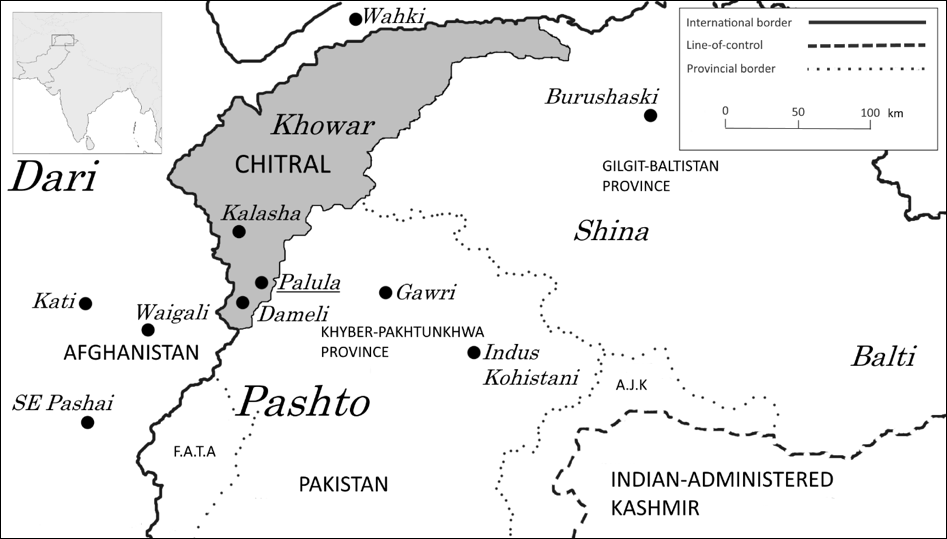
\includegraphics[width=\linewidth]{figures/liljegren-1}
  \caption{Chitral district and the surrounding region. Language names (only those that feature in the article) in italics.}
  \label{fig:hl1}
\end{figure}


There are only a few studies discussing evidentiality in this region, if we do not consider the observations made regarding the general pervasiveness of it in the grammars of Turkic and Sino-Tibetan, two of the genera represented here – although in a rather peripheral way, as we saw above. In a master’s thesis, \cite{Jones2009} analyses evidentiality and mirativity in Balti, and concludes that the language has a grammatical category of mirativity, reflected by present and past mirative markers, as well as a reportative verb suffix and some newly developed strategies for marking inference and supposition. 

Although evidentiality seems a less pervasive or significant feature in Iranian languages in general than is the case in Turkic and Sino-Tibetan, there are nevertheless indications that certain verb forms in the Persian varieties spoken in or near this region have epistemic uses. While the scope of epistemic uses is limited to past-time reference in Persian of Iran, \cite{Perry2000} presents evidence of much wider uses in Dari, i.e. the variety spoken in Afghanistan, encompassing quotative, inference, presumptive and speculative functions, in the present and future as well as in the past. \citeauthor{Bashir2006} also notes the use of a so-called “distant perfect” in Iranian Wakhi as a marker of inferentiality or mirativity (\citeyear{Bashir2006}; \citeyear[840]{Bashir2009}) and a second-position clitic in Pashto carrying out certain evidentiality-related functions (\citeyear{Bashir2006}).

Evidentiality distinctions in Indo-Aryan are in general not particularly significant or easily identifiable (\citealt[279--291]{Masica1991}; de \citealt{Haan2013}), but there are individual or areally significant exceptions, a fact noted by \cite{Bashir2006}. Khowar, the Indo-Aryan language mentioned above, and its closest relative Kalasha, are particularly interesting in this regard, as they may be part of an areal configuration, also including non-Indo-Aryan languages in the Hindukush-Karakoram region, where the semantic parameter of evidentiality to a varying extent has been grammaticalized (\citealt{Bashir1988}; \citeyear{Bashir1996a}; \citeyear{Bashir1996b}; \citeyear[823]{Bashir2003}; \citeyear{Bashir2010}). In another degree work, \cite{Lubberger2014} analyses a set of metarepresentation markers in Indus Kohistani — an Indo-Aryan language spoken in the central parts of the Hindukush-Karakoram region — of which at least two have a definite bearing on evidentiality. 

Based on previously, but severely limited, published research, \citeauthor{Bashir2006} also presents evidence for what she refers to as “robust inferential/indirective systems” (\citeyear{Bashir2006}) in several of the lesser-described Nuristani languages, as well as a special past-tense form only found in one of the dialects of Burushaski, which imparts an inferential-mirative meaning (\citeyear[14]{Bashir2010}). 


\section{Evidentiality and tense--aspect differentiation}\label{s:hl3}

The first evidential sub-system in Palula to be discussed, is that of verbal categories. Seven main TMA categories can be identified in the language (\citealt[247--263]{Liljegren2016}): four (Future, Present, Simple Past, Imperative) that are purely morphological categories, and another three that are periphrastically formed by the addition of auxiliaries (Past Imperfective, Perfect, Pluperfect). Palula is, like most other languages of the surrounding region, verb-final, and most frequently SOV. Verb morphology is suffixal, whether related to tense-aspect or agreement marking, and auxiliaries occur subsequent to the main verb.

Evidentiality is not a primary category in this system. Instead, the use of Simple Past vis-à-vis Perfect in Palula narratives often entails a contrast between direct and indirect evidence with events in the past. This is for instance reflected in the choice of verbal category when applying \citeauthor{Dahl1985}’s (\citeyear{Dahl1985}) TMA questionnaire. The event described in (‎\ref{ex:hl1}) is the speaker’s eye-witness account, whereas in ‎(\ref{ex:hl2}), it is what the speaker’s brother experienced and told the speaker prior to the moment of speaking that is being described. In the first case, the Simple Past (morphologically expressed with the perfective and ergative person/number agreement) is used. In the second case, the Perfect category (morphologically expressed with the perfective and the present tense form of a ‘be’-auxiliary, both agreeing in person/number with the O or S) is instead applied.

\begin{exe}
	\ex Palula -- Simple Past \label{ex:hl1}\\
	%\gll \textit{tíi} \textit{áa} \textit{báaṭ} \textit{uc̣h-i} \textit{ba} \textit{ǰhandra-í} \textit{the} \textit{uṛíit-u.} \textit{so} \textit{múṛ-u.}\\
	\gll tíi áa báaṭ uc̣h-i ba ǰhandra-í the \textbf{uṛíit-u} so \textbf{múṛ-u}\\
	{3\textsc{sg}.\textsc{rem}.\textsc{obl}} {\textsc{indf}} stone lift-\textsc{cvb} \textsc{top} snake-\textsc{obl} to {let.go.\textsc{pfv}-\textsc{msg}} {3.\textsc{sg}.\textsc{rem}.\textsc{nom}} {die.\textsc{pfv}-\textsc{msg}}\\
	\trans [This happened to my brother, I saw it:]‘He took a stone and threw it at the snake. It died.’ (PHL-TMAQ-NH:174–175)
\end{exe}

\begin{exe}
	\ex\label{ex:hl2} Palula -- Perfect\\
	%\gll \textit{tíi} \textit{áa} \textit{báaṭ} \textit{uc̣h-í} \textit{ba} \textit{ǰhandra-í} \textit{the} \textit{uṛíit-u} \textit{hín-u} \textit{ta}, \textit{so} \textit{múṛ-u} \textit{hín-u.}\\
	\gll tíi áa báaṭ uc̣h-í ba ǰhandra-í the \textbf{uṛíit-u} \textbf{hín-u} ta so \textbf{múṛ-u} \textbf{hín-u}\\
	{3\textsc{sg}.\textsc{rem}.\textsc{obl}} {\textsc{indf}} stone lift-\textsc{cvb} \textsc{top} snake-\textsc{obl} to {let.go.\textsc{pfv}-\textsc{msg}} {be.\textsc{prs}-\textsc{msg}} \textsc{sub} {3\textsc{sg}.\textsc{rem}.\textsc{nom}} {die.\textsc{pfv}-\textsc{msg}} {be.\textsc{prs}-\textsc{msg}} \\
	\trans [This happened to my brother, and he told me:]‘He took a stone and threw it at the snake. It died.’ (PHL-TMAQ-NH:179–180)
\end{exe}

The example in ‎(\ref{ex:hl3}) is from an interview, where the narrator tells how, a long time ago, he went to his father-in-law who told him a story. Here, the tense is the Simple Past. This can be compared with the corresponding Perfect forms used in the lines of ‎(\ref{ex:hl4}), belonging to a story about a boy named Katamosh who was told by his mother to go to his grandmother up in the high pastures. The latter is obviously part of a non-witnessed event with numerous components of fiction, such as animals acting and talking.

\begin{exe}
	\ex Palula -- Simple Past \label{ex:hl3}\\
	\gll áa deés táa \textbf{ɡúum} ta, máathe qisá \textbf{th-íil-u}\\
	one day there.\textsc{rem} go.\textsc{pfv}.\textsc{msg} \textsc{sub} 1\textsc{sg}.\textsc{dat} story do-\textsc{pfv}-\textsc{msg} \\
	\trans ‘One day I went there, and [he] told me a story.’ (PHL-Hunter:009)
\end{exe}

\begin{exe}
	\ex Palula -- Perfect \label{ex:hl4}\\
	\gll tasíi yéei taste áak ṭíki \textbf{th-íil-i} \textbf{hín-i} kaṭamúš ṭíki ḍóok-a pharé ɡhaṇḍ-í sóon-a dúši \textbf{ɡúum} \textbf{hín-u}\\
	3\textsc{sg}.\textsc{gen} mother 3\textsc{sg}.\textsc{dat} \textsc{indf} bread.cake do-\textsc{pfv}-\textsc{f} be.\textsc{prs}-\textsc{f} Katamosh bread.cake back-\textsc{obl} along tie-\textsc{cvb} pasture-\textsc{obl} toward go.\textsc{pfv}.\textsc{msg} be.\textsc{prs}-\textsc{msg}\\
	\trans ‘His mother made a cake of bread for him. Katamosh tied the bread to his back and set out to the high pastures.’ (PHL-Katamosh:009-010)
\end{exe}

However, it should be noted that this “extended” use of the Perfect is only a tendency, far from any obligatory marking of indirect evidence. It also seems that some authors or narrators are more prone than others to use it. In another, equally fantastic, story, an unnamed person in a distant past goes hunting, and while sitting down to eat the cooked meat of a markhor, a \textit{ṭhaaṭáaku}, a hairy and frightening creature suddenly appears. Here, however, as can be seen in ‎(\ref{ex:hl5}), the line of the narrative uses the Simple Past.

\begin{exe}
	\ex Palula -- Simple Past \label{ex:hl5}\\
	\gll anɡóor ǰeel-í táa pačaá kh-ainií široó \textbf{th-íil-u} široó \textbf{th-íil-u} ta tíi maǰí áa ǰhaṭíl-u ṭhaaṭáaku \textbf{yh-óol-u}\\
	fire light-\textsc{cvb} there.\textsc{rem} cook.\textsc{cvb} eat-\textsc{inf} starting do-\textsc{pfv}-\textsc{msg} starting do-\textsc{pfv}-\textsc{msg} \textsc{sub} 3\textsc{sg}.\textsc{rem}.\textsc{obl} in \textsc{indf} hairy-\textsc{msg} ogre come-\textsc{pfv}-\textsc{msg}\\
	\trans ‘When he had made a fire, he cooked the meat and started eating. Meanwhile, a \textit{ṭhaaṭáaku} suddenly appeared.’ (PHL-Thaataaku:004-005)
\end{exe}

An even less predictable contrast is that between Present and Future, as in ‎(\ref{ex:hl6}) and ‎(\ref{ex:hl7}), respectively. Both can be used with future-time reference. However, the choice in this case does not necessarily have a bearing on evidentiality per se. 

\begin{exe}
	\ex Palula -- Future \label{ex:hl6}\\
	\gll ma nis aáǰ \textbf{kh-úum} ta rhootašíi-a ba kanáa \textbf{bh-úum}\\
	1\textsc{sg}.\textsc{nom} 3\textsc{sg}.\textsc{prox}.\textsc{acc} today eat-1\textsc{sg} \textsc{sub} morning-\textsc{obl} \textsc{top} what become-1\textsc{sg}\\
	\trans ‘If I eat it today, what should I then do tomorrow?’ (PHL-HunterMonkey:005)
\end{exe}

\begin{exe}
	\ex Palula -- Present \label{ex:hl7}\\
	\gll uth-í maníit-u hín-u ki eé lhéṇḍu ɡóoi yh-óol-u ma tu \textbf{kha-áan-u}, muṣṭú ma thíi ráat \textbf{pil-áan-u} théeba ma thíi lhéṇḍ-i kakaríi \textbf{čap-áan-u}\\
	stand.up-\textsc{cvb} say.\textsc{pfv}-\textsc{msg} be.\textsc{prs}-\textsc{msg} \textsc{comp} o bald(\textsc{m}) where.from come-\textsc{pfv}-\textsc{msg} 1\textsc{sg}.\textsc{nom} 2\textsc{sg}.\textsc{nom} eat-\textsc{prs}-\textsc{msg} first 1\textsc{sg}.\textsc{nom} 2\textsc{sg}.\textsc{gen} blood drink-\textsc{prs}-\textsc{msg} then 1\textsc{sg}.\textsc{nom} 2\textsc{sg}.\textsc{gen} bald-\textsc{f} scalp gnaw-\textsc{prs}-\textsc{msg}\\
	\trans ‘I will eat you. First I will drink your blood, and then I will gnaw on your bald scalp.’ (PHL-Katamosh:030–032)
\end{exe}

When on the other hand two present-time referring utterances are being contrasted as in ‎(\ref{ex:hl8}) and ‎(\ref{ex:hl9}), there is a clearer correspondence between the use of Present and direct evidence, on the one hand, and the use of Future and indirect evidence, on the other.

\begin{exe}
	\ex Palula -- Present \label{ex:hl8}\\
	\gll faríd teeṇíi ɡhooṣṭ-á \textbf{hín-u}\\
	Farid \textsc{refl} house-\textsc{obl} be.\textsc{prs}-\textsc{msg} \\
	\trans ‘Farid is at home [I was there and saw him].’ (PHL-20157027-elic:007)
\end{exe}


\begin{exe}
	\ex Palula -- Future \label{ex:hl9}\\
	\gll faríd teeṇíi ɡhooṣṭ-á \textbf{hóons-a}\\
	Farid \textsc{refl} house-\textsc{obl} be-3\textsc{sg}\\
	\trans ‘Farid is at home [he is usually at this time].’ (PHL-20157027-elic:008)
\end{exe}


\section{Evidentiality and utterance-final mood markers}\label{s:hl4}

Palula has a closed set of markers that one way or another specify the relationship between an utterance as a whole and the speaker and/or hearer, e.g. signaling a polar question or a request. Almost exclusively, such mood markers occur utterance-finally, i.e. in most cases following the finite verb. At least three of those markers have functions related to, or partly related to, evidentiality.

The most frequent (in my corpus) of the three, \textit{thaní}, is a quotative (\citealt[267, 377–387]{Liljegren2016}). In Palula narratives, it usually marks — or closes — directly quoted speech, as in ‎(\ref{ex:hl10}).

% error messages?!
\begin{exe}
	\ex Palula -- quotative \label{ex:hl10}\\
	\gll so ba maidóon-a=wée be ba áa khur raál the ba kar kar kar gír-a koó hín-ee yh-óoi \textbf{thaní}\\
	3\textsc{msg}.\textsc{nom} \textsc{top} field-\textsc{obl}=into go.\textsc{cvb} \textsc{top} one foot High do.\textsc{cvb} \textsc{top} around around around turn-3\textsc{sg} who be.\textsc{prs}-\textsc{mpl}.\textsc{q} come-\textsc{imp}.\textsc{pl} \textsc{quot}\\
	\trans ‘He was spinning around and around in the field, holding up one leg, [and he was calling out, \textit{saying},]``Is there anyone here [brave enough]? Come on!''’ (PHL-JangibazKhan:037–038)
\end{exe}

However, it may occasionally extend into (non-uttered) reported thought, as shown in ‎(\ref{ex:hl11}), here used along with a preposed \textit{ki}-complementizer.

\begin{exe}
	\ex Palula -- quotative \label{ex:hl11}\\
	\gll ɡhrast-á karáaṛ-a asíi xiaál \textbf{ki} ɡóo mheer-íl-u heentá kh-óol-u \textbf{thaní}\\
	wolf-\textsc{obl} leopard-\textsc{obl} 1\textsc{pl}.\textsc{gen} opinion \textsc{comp} maybe kill-\textsc{pfv}-\textsc{msg} \textsc{condl} eat-\textsc{pfv}-\textsc{msg} \textsc{quot}\\
	\trans ‘We thought that perhaps a leopard or a wolf had killed and eaten him.’ (PHL-GhaziSamad:011)
\end{exe}

If an explicit PCU (perception-cognition-utterance) predicate precedes the complement, the use of the quotative is more variable. In ‎(\ref{ex:hl12}), where the utterance predicate \textit{ṭeekílu} ‘called (out)’ is used, there is no closing \textit{thaní}, while in ‎(\ref{ex:hl13}), the quotative \textit{thaní} is co-occurring with the preceding predicate of knowledge acquisition, \textit{búda hína} ‘(have) understood’.

\begin{exe}
	\ex Palula -- utterance without quotative \label{ex:hl12}\\
	\gll áak šúma ṭeek-íl-u ée kúṛi thíi míiš-i paaṇṭí ṣ-éel-i hín-i tu míiš ba na\\
	\textsc{indf} parrot.\textsc{obl} call-\textsc{pfv-msg} o woman \textsc{2sg.gen} man-\textsc{gen} clothes dress-\textsc{pfv-f} be.\textsc{prs-f} 2\textsc{sg.nom} man \textsc{top} \textsc{neg}\\
	\trans ‘A parrot called out: “O woman, you have dressed like a man, but you are not a man.’ (PHL-WiseMinister:012-013)
\end{exe}

\begin{exe}
	\ex Palula -- utterance with PCU predicate and quotative \label{ex:hl13}\\
	\gll búd-a hín-a ki phaí wíi-a ɡíi thaní\\
	understand.\textsc{pfv}-\textsc{mpl}  be.\textsc{prs}-\textsc{mpl} \textsc{comp} girl water-\textsc{obl} go.\textsc{pfv}.\textsc{fsg} \textsc{quot}\\
	\trans ‘They understood that the girl must have thrown herself into the water.’ (PHL-ShepherdBoy:060)
\end{exe}


Another, highly grammaticalized, function of \textit{thaní} is when it occurs postposed to a proper noun and carries the meaning ‘called, thus named’, referring to the immediately preceding noun. An example is provided in ‎(\ref{ex:hl14}).


\begin{exe}
	\ex Palula -- `name' \label{ex:hl14}\\
	\gll miír \textbf{thaní} áak míiš heens-íl-u de\\
	Mir \textsc{quot} \textsc{indf} man exist-\textsc{pfv}-\textsc{msg} \textsc{pst}\\
	\trans ‘There was a man \textit{called} Mir.’ (PHL-GhaziSamad:051)
\end{exe}

Hearsay can be (but is not necessarily) marked with an utterance-final \textit{maní}. The reported content, preceding it, is in such cases often mythical or unexpected, as in ‎(\ref{ex:hl15}).

\begin{exe}
	\ex Palula -- hearsay \label{ex:hl15}\\
	\gll dac̣h-áan-u ta eeteeṇ-ú=ee áak šay yh-óol-u \textbf{maní} maaxustán de \textbf{maní} áa šay yh-óol-u babár búd-u ki na\\
	look-\textsc{prs}-\textsc{msg} \textsc{sub} such-\textsc{msg}=\textsc{conj} \textsc{indf} thing come-\textsc{pfv}-\textsc{msg} \textsc{hsay} evening be.\textsc{pst} \textsc{hsay} \textsc{indf} thing come-\textsc{pfv}-\textsc{msg} furry.thing understand.\textsc{pfv}-\textsc{msg} or \textsc{neg}\\
	\trans ‘Then a creature appeared, it is said, in the evening, it is said, a furry one, you know, don’t you.’ (PHL-AyanMir1:065)
\end{exe}

However, the use of \textit{maní} is not restricted to narrative discourse. It is also used in everyday conversation, as in ‎(\ref{ex:hl16}), an excerpt from an online chat conversation. It should be noted that it is only the first of the two clauses that is hearsay-marked.

\begin{exe}
	\ex Palula -- hearsay \label{ex:hl16}\\
	\gll asíi atshareet-á bíiḍ-u kir dít-u hín-u \textbf{maní} hiimeel-í bi whéet-im hín-i\\
	1\textsc{pl}.\textsc{gen} Ashret-\textsc{obl} much-\textsc{msg} snow fall.\textsc{pfv}-\textsc{msg} be.\textsc{prs}-\textsc{msg} \textsc{hsay} glacier-\textsc{pl} \textsc{sep} come.down.\textsc{pfv}-\textsc{fpl} be.\textsc{prs}-\textsc{f}\\
	\trans ‘[I have been told that] a lot of snow has fallen in our [village] Ashret, and there have been avalanches as well.’ (PHL-CHN070320)
\end{exe}

Finally, a third, and in the present corpus much more infrequently occurring marker, \textit{ɡa}, signals inferred, presumed or assumed knowledge, as in ‎(\ref{ex:hl17}).

\begin{exe}
	\ex Palula -- assumption \label{ex:hl17}\\
	\gll anú dhút-a de baaǰá bhanǰa-áan-a eetáai aawaáz yh-áand-u eh rueeleé hín-a \textbf{ɡa} rueeleé ba aní sarkaarí sipaahi-aán hóons-an de\\
	\textsc{prox}.\textsc{nom}.\textsc{msg} mouth-\textsc{obl} give.\textsc{cvb} harmonium beat-\textsc{prs}-\textsc{mpl} from.there sound come-\textsc{prs}-\textsc{msg} oh government.official.\textsc{pl} be.\textsc{prs}-\textsc{mpl} \textsc{ass} government.official.\textsc{pl} \textsc{top} \textsc{prox} official soldier-\textsc{pl} exist-3\textsc{pl} \textsc{pst}\\
	\trans ‘I heard a sound like a harmonium being played. “Oh,” I thought, “These must be government officials, such professional soldiers they are.”’ (PHL-Hunter:067-068)
\end{exe}


\section{Evidentiality and second-position discourse particles}\label{s:hl5}

Palula discourse markers are second-position clitics that specify the discourse role of a preceding unit (often a noun phrase) in relation to adjacent units. A secondary effect of some discourse markers is that they indicate how larger units (e.g. clauses) are interrelated, especially when used in pairs, or when the same marker is used repeatedly in two adjacent clauses. The latter use overlaps with the function of conjunctions.
 
The particle \textit{xu} is such a second-position clitic. It signals surprise, as in ‎(\ref{ex:hl18}), or emphasis, occurring postposed to the first-position constituent that is thus being focused. While it is often difficult to find good translation equivalents in English, it is strikingly similar in meaning to the Swedish modal particles \textit{ju} or \textit{visst}.

\begin{exe}
	\ex Palula -- assumption \label{ex:hl18}\\
	\gll ée míi xudaáyaa ni \textbf{xu} ux-íi rhaíi hín-i\\
	o 1\textsc{sg}.\textsc{gen} my.God 3\textsc{pl}.\textsc{prox}.\textsc{nom} \textsc{emph} camel-\textsc{gen} footprints be.\textsc{prs}-\textsc{f}\\
	\trans ‘O my God, it’s the footprints of a camel.’ (PHL-Hunter:061) [Swedish: ‘Men herregud, det är ju kamelspår!’]
\end{exe}

Other members of the set of second-position discourse particles are: \textit{bi} (separation marker, see \ref{ex:hl16} for an example), \textit{ba} (switch-topic marker), \textit{ta} (contrast marker), \textit{ee} (amplification marker). The extremely frequently occurring switch-topic marker \textit{ba}, is for instance used to make a contrast with an immediately preceding subject explicit, as in ‎(\ref{ex:hl19}), but has a number of other functions, some of them challenging to define exactly (\citealt[419--425]{Liljegren2016}). (See \ref{ex:hl6} for another example of the contrastive function.) 

\begin{exe}
	\ex Palula -- contrast \label{ex:hl19}\\
	\gll míi ɡhoóṣṭ lookúṛi hín-u, iskuúl \textbf{ba} asíi kaṇeeɡhaá hín-i\\
	1\textsc{sg}.\textsc{gen} house {Lokuri [place]} be.\textsc{prs}-\textsc{msg} school \textsc{top} 1\textsc{pl}.\textsc{gen} {Kanegha [place]} be.\textsc{prs}-\textsc{f}\\
	\trans ‘My house is in Lokuri, while our school is in Kanegha.’ (PHL-Our school:004)
\end{exe}


\section{Origins and grammaticalization paths}\label{s:hl6}

As for the contrastive use of tense-aspect categories to signal indirect vs. direct evidence, there is evidence of a similar-functioning differentiation in Old Indo-Aryan, i.e. in the ancestral language (or a closely related language to that) of Palula and other modern-day Indo-Aryan languages. In the system described by the Indian grammarian Pāṇini, there were three categories with past-time reference: Aorist, Imperfect and Perfect. Of these three, the Perfect was used with special reference to reported, less recent, events, that is excluding the speaker’s direct witnessing the event reported, while the Imperfective had the same time reference as the Perfect but implied that the speaker was indeed a direct witness. The Aorist, which functioned as a more general past tense, was the only one of the three that could refer to recent events (\citealt[235]{Cardona2002}). \cite[62]{Deshpande1981} summarizes, in the same vein, this three-way contrast as: a) [+past +recent +/-seen] (Aorist), b) [+past -recent +seen] (Imperfective), and c) [+past -recent -seen] (Perfect), thus making the presence or absence of a [seen] feature the minimal contrast between the latter two, a distinction that \cite{Bashir2006} argues has been passed on to some of the descendant languages, the two Chitral languages Kalasha and Khowar in particular.  

In Khowar, which is locally influential in the district where Palula is spoken, and also is the second language of many Palula speakers, the distinction between indirect evidence [+past -seen] and direct evidence [+past +seen] is upheld in the tense-aspect system (which has retained forms that were lost in most other Indo-Aryan languages), as can be seen in comparing ‎(\ref{ex:hl20}) with ‎(\ref{ex:hl21}). Here, the [-seen] value of the Past Inferential is further specified with a \textit{birai} (a past participle of ‘become’ whose epistemic function has developed later) which adds a mirative meaning to the reported event. The encoding of such evidentiality-related differentiation, is non-optional in Khowar (\citealt[221–222]{Bashir2007}).

\newpage
\begin{exe}
	\ex Khowar – Past Actual \label{ex:hl20}\\
	\gll hase boht-o ɡan-i ayi-o ṭek-o \textbf{lak-it-ai} hase \textbf{o-br-it-ai}\\
	3\textsc{sg}.\textsc{rem}.\textsc{nom} stone-\textsc{obl} take-\textsc{cvb} snake-\textsc{obl} \textsc{top}-\textsc{obl} let.go-\textsc{pst}-3\textsc{sg} 3\textsc{sg}.\textsc{rem}.\textsc{nom} \textsc{pst}-die-\textsc{pst}-3\textsc{sg}\\
	\trans [This happened to my brother, I saw it:] ‘He took a stone and threw it at the snake. It died.’ (KHW-TMAQ-AA:174-175)
\end{exe}

\begin{exe}
	\ex Khowar – Past Perfective Inferential \label{ex:hl21}\\
	\gll hase boht-o ɡan-i ayi-o ṭek-o \textbf{lak-iru} \textbf{bir-ai} hase \textbf{birdu} \textbf{bir-ai}\\
	3\textsc{sg}.\textsc{rem}.\textsc{nom} stone-\textsc{obl} take-\textsc{cvb} snake-\textsc{obl} \textsc{top}-\textsc{obl} let.go-\textsc{pptc} become.\textsc{pst}.\textsc{infer}-3\textsc{sg} 3\textsc{sg}.\textsc{rem}.\textsc{nom} die.\textsc{pptc} become. \textsc{pst}.\textsc{infer}-3\textsc{sg}\\
	\trans [This happened to my brother, and he told me:] ‘He took a stone and threw it at the snake. It died.’ (KHW-TMAQ-AA:179-180) 
\end{exe}


Very similar distinctions are being made in the Kalasha tense-aspect system. For instance, two distinct past-time referring forms of ‘were’ are used. In ‎(\ref{ex:hl22}), the past actual \textit{asini} is used as the speaker points to the domestic animals as witnessed entities in the real world. In ‎(\ref{ex:hl23}), the past inferential \textit{asta} instead is used, as a means for the narrator to portray the participants in the story as the creations of fiction.

\begin{exe}
\ex Kalasha -- Past Actual \label{ex:hl22}\\
	\gll tara \textbf{as-ini} ɡak tara ɡordok hãš\\
	there.\textsc{rem}.\textsc{spc} be.\textsc{pst}.\textsc{act}-3\textsc{pl} cow there.\textsc{rem}.\textsc{spc} donkey horse\\
	\trans ‘There were cows, donkeys and horses there.’  (\citealt[136]{Heegard2015}) 
\end{exe}

\begin{exe}
\ex Kalasha -- Past Perfective Inferential \label{ex:hl23}\\
	\gll ek ɬawak ek  šara malɡiri \textbf{asta}\\
	one fox one markhor friend be.\textsc{pst}.\textsc{infer}.3\\
	\trans ‘Once a fox and a markhor were friends.’ (\citealt[182]{Heegard2015}) 
\end{exe}

Kalasha is not a common second language of Palula speakers. However, considerable interaction apparently took place between the communities in the past, and there is reason to believe that Kalasha, at least in part of what is now Palula-speaking territory, is exerting substratal influence, as conversions from the traditional Kalasha religion often resulted in a gradual language shift from Kalasha to one of the surrounding languages spoken by a Muslim majority population, Palula in those days being one of the main candidates (\citealt[117--118]{Cacopardo2001}; \citealt[55--60]{Decker1992}).

Although the distinction in Palula also could have been inherited, it is equally probable to have been areally influenced and/or reinforced. Apart from evidential\-ity-related distinctions in the verbal systems of Khowar and Kalasha, a few other languages in the immediate region reflect similar contrasts in their TMA systems. There are for instance epistemic verb forms in regionally influential Persian varieties (\citealt{Perry2000}; \citealt[461]{WindfuhrPerry2009}). \citeauthor{Bashir2010} (\citeyear[14–15]{Bashir2010}; \citeyear[839]{Bashir2009}) also mentions the perfect in the Iranian language Wakhi as well as in Tajik Persian as specifically correlated to indirect evidence. Another possible parallel is the contrastive use of a proximate vs. a distal perfect in Pashai, another Indo-Aryan language (or perhaps more correctly, group of related language varieties), spoken across the border in northeastern Afghanistan (\citealt[295--297]{Lehr2014}). Perhaps this, in turn, is part of a considerably larger areal configuration in Western and Central Asia, something that \citeauthor{Dahl1985} (\citeyear[152]{Dahl1985}) is hinting at, when he describes the extension of perfects into the realm of quotatives as an areal phenomenon with an approximate geographical correlation with the former Ottoman Empire (including e.g. Kurdish and Turkish), but it goes without saying that the secondary use of perfects for such functions has indeed been verified cross-linguistically much farther afield (\citealt[112]{Aikhenvald2004}).

As for the mood markers described in Section ‎\ref{s:hl4}, they are to a varying extent grammaticalized in Palula, which is reflected in the textual occurrence of these markers (\tabref{tab:hl1}). It should be noted, however, that identical forms may occur in other uses in the material.


\begin{table}
\begin{tabularx}{\textwidth}{lYrYr}
\lsptoprule
& \textbf{Utterance-final} & \textbf{In other uses} & \textbf{As other verb forms} & \textbf{Total}\\
\midrule
   \textit{thaní} & 117 & 51 & 109 & 277\\
	\textit{maní} & 61 & 14 & 351 & 426\\
	\textit{ɡa} & 20 & 117 & - & 137\\
\lspbottomrule
\end{tabularx}
\caption{Text occurrences of \textit{thaní}, \textit{maní} and \textit{ɡa}, and of forms related to them. (In a text corpus consisting of 76 transcribed and annotated Palula texts, mainly narrative.)}
 \label{tab:hl1}
\end{table}	


The quotative marker \textit{thaní} is the most frequent of the three. The relatively frequent occurrence of the same form but in other uses is largely accounted for by its post-nominal “naming” function, as shown in example ‎‎(\ref{ex:hl14}) above. It is highly grammaticalized as a quotative, but its co-occurrence with a preposed (and “borrowed”) \textit{ki}-complementizer, on the one hand, and the alternative construction with \textit{ki} altogether lacking an quote-final \textit{thaní}, as in ‎(\ref{ex:hl24}), on the other hand, points to an ongoing competition with the “new” Persian-derived \textit{ki}-strategy (further reinforced by the corresponding construction in Urdu), in which the \textit{thaní}-less construction most likely is winning out in the long run: …\textit{thaní} (as in \ref{ex:hl10}) > \textit{ki}...\textit{thaní} (as in \ref{ex:hl11}) > \textit{ki}... A similar development has been observed in neighbouring Kalasha with regard to the indigenous utterance-final \textit{ɡhõi} and the “imported” utterance-initial \textit{ki} (\citealt[266--324]{Bashir1988}).

\begin{exe}
\ex Palula -- quotative \label{ex:hl24}\\
	\gll dun-áaṭ-u bh-íl-u hín-u \textbf{ki} aní ba kateeeṇ-í ǰuánd\\
	think-\textsc{ag}-\textsc{msg} become-\textsc{pfv}-\textsc{msg} be.\textsc{prs}-\textsc{msg} \textsc{comp} 3\textsc{fsg}.\textsc{prox}.\textsc{nom} \textsc{top} what.kind-\textsc{f} life\\
	\trans ‘He started thinking, “What a life!”’(PHL-Katamosh:057) 
\end{exe}


Formally, \textit{thaní} is a converb form (or conjunctive participle) of the verb \textit{thané}- ‘call, say’. In contemporary Palula, few other forms of that verb are in fact in use, once more confirming the level of grammaticalization that this converb has reached. \cite{Bashir1996a} found in a study of \textsc{say}-quotatives, and similarly derived markers, that they are present in many of the region’s languages (and beyond), and argues for areal convergence. Examples of such markers include: Indus Kohistani (Indo-Aryan) \textit{karee} (\citealt[67--69]{Lubberger2014}); Kalasha (Indo-Aryan) \textit{ɡhõi} (\citealt[67]{Heegard2015}); Khowar (Indo-Aryan) \textit{reé} (\citealt[225--235]{Bashir1996a}); Gawri (Indo-Aryan) \textit{är(o)} (\citealt[147--149]{Baart1999}); Dameli (Indo-Aryan) \textit{ɡani} (\citealt[176--177]{Perder2013}); Gilgiti Shina (Indo-Aryan) \textit{theé} (\citealt[28]{RadloffShakil1998}); Balti (Sino-Tibetan) \textit{zer}/\textit{zere} (\citealt[270]{Bashir1996a}; \citealt[64]{Jones2009}); and possibly Burushaski (isolate) \textit{nusé(n)} (\citealt[262]{Bashir1996a}), although a pre-posed \textit{ke} is the preferred marker of direct speech (\citealt[193]{Berger1998}). While many of them are indeed grammaticalized forms of a verb with the meaning ‘say’, a number of them are instead ultimately related to a ‘do’-verb; that is likely the case with Palula \textit{thaní} (cf. \textit{the}- ‘do’), the corresponding markers in other Shina varieties, as well as Indus Kohistani \textit{karee} (< \textit{kar}- ‘do’).
 
Dameli is another geographically close neighbour of Palula, spoken in the next valley to the south. Here, too, the quotative, which is derived from a converb of ‘say’, is extended to predicates of cognition, as in ‎(\ref{ex:hl25}), and additionally is postpositioned to a noun phrase with the meaning ‘called, thus named’, as in ‎(\ref{ex:hl26}), just like in Palula. 

\newpage
\begin{exe}
\ex Dameli -- quotative \label{ex:hl25}\\
	\gll mããtẽẽ dac̣i-na mãã-i tukuri kii ɡiɡ-een \textbf{ɡani}\\
	around see-\textsc{ipfv}.3\textsc{msg} 1\textsc{sg}.\textsc{poss}-\textsc{f} basket who take-\textsc{pfv}.3\textsc{pl} \textsc{quot}\\
	\trans ‘He looks around, thinking, “Who took my basket?”’ (\citealt[176]{Perder2013}) 
\end{exe}

\begin{exe}
\ex Dameli – ‘called’ \label{ex:hl26}\\
	\gll aats-i baloo daaš \textbf{ɡani} ek baaṭ daro\\
	come-\textsc{cvb} big rock \textsc{quot} one stone \textsc{cop}.\textsc{inan}.\textsc{ipfv}.3\\
	\trans ‘Having come there, there is a big stone called the great rock.’ (\citealt[177]{Perder2013}) 
\end{exe}

The Palula hearsay marker \textit{maní}, is of lower frequency in the text corpus, and is possibly grammaticalized to a lesser extent than \textit{thaní}. When it is used it is often in order to emphasize the non-witnessed, and often questionable (in the mind of the speaker), character of the particular event or situation thus marked, rather than to signal just any instance of reported speech or hearsay. Note that \textit{maní} in ‎(\ref{ex:hl27}) only occurs after the second finite verb of this utterance, not after the first.

\begin{exe}
\ex Palula -- hearsay \label{ex:hl27}\\
	\gll eesé baačaá-ii bóoš zára kuṛíina heens-íl-im de tasíi áaṣṭ zára kuṇaak-á heens-íl-a de \textbf{maní}\\
	\textsc{rem} king-\textsc{gen} twelve thousand.\textsc{pl} women.\textsc{pl} live-\textsc{pfv}-\textsc{fpl} \textsc{pst} 3\textsc{sg}.\textsc{gen} eight thousand.\textsc{pl} child-\textsc{pl} live-\textsc{pfv}-\textsc{mpl} \textsc{pst} \textsc{hsay}\\
	\trans ‘This king had twelve thousand wives, and is said to have had eight thousand children.’ (PHL-AboutAKing:007-008) 
\end{exe}

The marker \textit{maní} is like \textit{thaní} derived from a converb, in this case of the verb \textit{mané}- ‘speak, recite, say’. In the corpus, quite a number of other uses of this verb occur, including a few instances of it as a non-grammaticalized converb, entirely homophonous with the hearsay marker. An example of the latter is seen in ‎(\ref{ex:hl28}), where \textit{maní} heads a subordinate clause with a subsequence reading, thus repeating the preceding lexical finite verb ‘said’ in its converb form ‘having said’, simply corresponding to ‘then’ in English.

\begin{exe}
\ex Palula -- maní as converb \label{ex:hl28}\\
	\gll íṇc̣-a maníit-u hín-u ki  šóo ba tu thulí wháat-u heentá ma tu kh-úum eendáa \textbf{man-í} ba iṇc̣ áak keeṇ-í šíiṭi the ɡúum hín-u\\
	bear-\textsc{obl} say.\textsc{pfv}-\textsc{msg} be.\textsc{prs}-\textsc{msg} \textsc{comp} good.\textsc{msg} \textsc{top} 2\textsc{sg}.\textsc{nom} fattened come.down.\textsc{pfv}-\textsc{msg} \textsc{condl} 1\textsc{sg}.\textsc{nom} 2\textsc{sg}.\textsc{nom} eat-1\textsc{sg} like.that say-\textsc{cvb} \textsc{top} bear \textsc{indf} cave-\textsc{obl} inside to go.\textsc{pfv}.\textsc{msg} be.\textsc{prs}-\textsc{msg}\\
	\trans ‘The bear said: “Good, if you come down fattened I will eat you.” Then [lit. Having said that,] the bear went into a cave.’ (PHL-Katamosh:025-026) 
\end{exe}

Reportative markers with similar functions (and in many cases with a similar history) have been noted for other languages in the region, e.g. Indus Kohistani \textit{lee} (\citealt[22--23]{Lubberger2014}); Kati (Nuristani) \textit{mem} (\citealt{Strand2016}); Waigali (Nuristani) -\textit{le} (\citealt[173–182]{Degener1998}); and Balti/Purik (Sino-Tibetan) -\textit{lo} (\citealt[57--62]{Jones2009}; \citealt[776--792]{Zemp2013}).

In the example from Indus Kohistani in ‎(\ref{ex:hl29}), the speaker quotes one of her sons speaking to her at the time when he had come home after the big earthquake in 2005. The reportative \textit{lee} cliticizes to the finite verb in each of the two clauses.

\begin{exe}
\ex Indus Kohistani -- reportative \label{ex:hl29}\\
	\gll iskul-ãĩ kùṛ-muṛ bazíthe=lee hãã maasmá búṭ báč hu-úthe=lee\\
	school-\textsc{gen}.\textsc{f} wall.\textsc{fpl}-\textsc{echo} go.\textsc{prs}.\textsc{pfv}.\textsc{mpl}=\textsc{hsay} and child.\textsc{pl} all saved become-\textsc{prs}.\textsc{pfv}.\textsc{mpl}=\textsc{hsay}\\
	\trans ‘The walls of the school and stuff went down, but the children all escaped.’ (\citealt[26--27]{Lubberger2014})
\end{exe}

There are only a few, and in some cases rather dubious, instances of \textit{ɡa} as an utterance-final marker of inferentiality in the Palula corpus. It is most likely related to the homophonous indefinite-interrogative pronoun \textit{ɡa} ‘what, any, what kind of, any kind of’. Probably, it was first used in the utterance-final position as a tag. The assumption here is that it is even less grammaticalized or established than \textit{maní} and remains somewhat varying in its application: as a request for confirmation, marking suspense or surprise, etc. The particle \textit{bo} in Kohistani Shina, see example in ‎(\ref{ex:hl30}), has similar semantics and distribution (\citealt[204]{SchmidtKohistani2008}).

\begin{exe}
\ex Kohistani Shina -- presumption \label{ex:hl30}\\
	\gll mi qǽæs ǰo kudí múṭho khári níiz-iǰ-aan-o \textbf{bo}\\
	my guess some where tree under sleep-\textsc{absp}-is-3\textsc{msg} \textsc{ass}\\
	\trans ‘I guess he must be asleep under a tree somewhere.’ (\citealt[204]{SchmidtKohistani2008})
\end{exe}

Careful elicitation (in ‎\ref{ex:hl31}), in which imaginary situations were described, confirms the emerging paradigmatic contrast \textsc{zero} vs. \textit{maní} vs. \textit{ɡa} as corresponding to a) an event directly observed by the speaker, b) an event heard about but not seen by the speaker c) an inference/assumption on the part of the speaker.

\begin{exe}
\ex Palula minimal contrastsː direct (a) vs. hearsay (b) vs. inference/assumption (c) \label{ex:hl31}
	\begin{xlist}
	\ex 
	\gll kir  dít-u hín-u\\
	snow put.\textsc{pfv}-\textsc{msg} be.\textsc{prs}-\textsc{msg}\\
	\trans ‘It has snowed.’ [directly observed] (PHL-20157027-elic:001)
	\ex 
	\gll kir dít-u hín-u \textbf{maní}\\
	snow put.\textsc{pfv}-\textsc{msg} be.\textsc{prs}-\textsc{msg} \textsc{hsay}\\
	\trans ‘It has snowed.’ [not seen but heard from sb else] (PHL-20157027-elic:002)
	\ex 
	\gll kir dít-u hín-u \textbf{ɡa}\\
	snow {put.\textsc{pfv-msg}} {be.\textsc{prs-msg}} {\textsc{infer}}\\
	\trans ‘It has snowed.’ [not directly observed but inferred from other evidence, e.g. snow on somebody else’s boots] (PHL-20157027-elic:003)
	\end{xlist}
\end{exe}

Interestingly, the same elicitation task resulted in a two-way differentiation in neighbouring Khowar ‎(\ref{ex:hl32}).

\begin{exe}
\ex Khowar minimal contrastː direct (a) vs. hearsay (b)/assumption (c) \label{ex:hl32}
	\begin{xlist}
	\ex 
	\gll him \textbf{arer} /  him \textbf{kor-i} \textbf{šer}\\
	snow do.\textsc{pst}.3\textsc{sg} {} snow do-\textsc{cvb} be.\textsc{inan}.\textsc{prs}.\textsc{act}\\
	\trans ‘It has snowed.’ [directly observed] (KHW-20157027-elic:001)
	\ex 
	\gll him \textbf{kardu} \textbf{bir-ai}\\
	snow do.\textsc{pptc} become.\textsc{pst}.\textsc{infer}-3\textsc{sg}\\
	\trans ‘It has snowed.’ [not seen but heard from sb else] (KHW-20157027-elic:002)
	\ex 
	\gll him \textbf{kardu} \textbf{bir-ai}\\
	snow do.\textsc{pptc} become.\textsc{pst.infer}-3\textsc{sg}\\
	\trans ‘It has snowed.’ [not directly observed but inferred from other evidence, e.g. snow on somebody else’s boots] (KHW-20157027-elic:003)
	\end{xlist}
\end{exe}

The discourse particle \textit{xu} is most likely a loan from Pashto. In Pashto, \textit{xo} is used as an emphatic particle (a second position clitic), with the approximate meaning ‘in fact’. In Pashto as well as in Palula \textit{xo}/\textit{xu} is homophonous, or alternatively polysemous, with a clause-initial adversative conjunction ‘but’. The examples in ‎(\ref{ex:hl33}) and ‎(\ref{ex:hl34}) illustrate the strikingly similar uses and clause positions of the particle in the two languages.


\begin{exe}
\ex Palula -- use of the particle \textit{xu} \label{ex:hl33}\\
	\gll lo tu keé kh-óo lo \textbf{xu} thíi bhróo atsharíit-u thíi qóom\\
	3\textsc{msg}.\textsc{dist}.\textsc{nom} 2\textsc{sg}.\textsc{nom} why eat-3\textsc{sg} 3\textsc{msg}.\textsc{dist}.\textsc{nom} \textsc{emph} 2\textsc{sg}.\textsc{gen} brother Ashreti-\textsc{msg} 2\textsc{sg}.\textsc{gen} tribe\\
	\trans ‘Why would he eat you? He is your Ashreti brother and of your own tribe.’ (PHL-GhaziSamad:019-020)
\end{exe}

\begin{exe}
\ex Pashto -- use of the particle \textit{xo} \label{ex:hl34}\\
	\gll dā \textbf{xo} zmā wror day də bel saṛ-i wror na\\
	this.\textsc{dir} \textsc{emph} 1\textsc{sg}.\textsc{gen} brother be.\textsc{prs}.3\textsc{msg} of other man-\textsc{obl} brother \textsc{neg}\\
	\trans ‘He is in fact my brother, not some other man’s brother.’ (\citealt[375]{David2013})
\end{exe}

A parallel pattern of use has also been reported for \textit{xu} in Dameli, another neighbouring Indo-Aryan language (\citealt[168]{Perder2013}), and similar sets of particles in many languages in the region (especially to the west) have been described, for instance in Nuristani Waigali by \cite[166--188]{Degener1998} and Indo-Aryan Gawri (\citealt[159--166]{Baart1999}). \citeauthor{Degener1998} describes one of the particles in Waigali, \textit{be}, as for instance signalling empathy or some pre-understanding for a particular situation that has arisen. In the example in ‎(\ref{ex:hl35}), there is also a component of reproach, again difficult to find a good equivalent for in English but somewhat easier in German (which like Swedish has its own set of modal particles); \textit{be} frequently corresponds to German \textit{doch}, but in individual examples \citeauthor{Degener1998} also offers the translations \textit{bloß}, \textit{aber}, \textit{bestimmt}, \textit{also}, \textit{nun}.  Some of those uses seem to overlap with Palula \textit{xu}, others with \textit{ba}.

\largerpage[1.5]
\begin{exe}
\ex Waigali -- use of the particle \textit{be} \label{ex:hl35}\\
	\gll yi manaṣa \textbf{be} ämeba pũt süräy\\
	this man \textsc{empt} 1\textsc{pl}.\textsc{gen} way blocked\\
	\trans ‘This man has apparently blocked our way. [Dieser Mann hat \textit{doch} unseren Weg versperrt!]’ (\citealt[167]{Degener1998})\footnote{No morpheme glossing is provided in the source, only a free translation of the sentence as a whole. The glossing and the English translation are my own.}
\end{exe}
\clearpage

There is evidence for a relatively high degree of “borrowability” across languages (\citealt{Svard2014}; \citealt{LiljegrenSvard2017}; \citealt[183–184]{Perder2013}) with these types of markers, pointing e.g. to a possible diachronic link between Waigali \textit{be} and Dameli/Palula \textit{ba}. Probably, the use of such modal or discourse particles is a relatively new strategy of signalling evidentiality and inferentiality as far as Palula is concerned.

\section{Summary}\label{s:hl7}

Evidential marking and evidentiality-related distinctions in Palula are, like in many Indo-Aryan languages, observable in so-called scattered coding. It is not forming an independent system, and it is often optional or comes about as a secondary effect of the coding of other main functions. It is most obviously reflected in three separate parts of the language system, namely a) as a component, or byproduct, of tense—aspect differentiation, b) by a subset of utterance-final mood markers, and c) by (at least) one member of a set of second-position discourse particles. In the case of tense—aspect, the choice between a simple past and a perfect, when referring to a past-time event, is at least partly correlated with direct (witnessed) vs. indirect (non-witnessed) evidence. A less stable correlation for present-time reference can be observed between the use of present tense and direct evidence, and between the use of future tense and indirect evidence.  Three mood markers have epistemic functions: \textit{thaní} is a quotative; \textit{maní} is a hearsay (or possibly mirativity) marker; and \textit{ɡa} indicates inferred or assumed knowledge, although the latter seems only marginally grammaticalized. The second-position discourse marker \textit{xu} signals surprise or emphasis.

As for tense-aspect and its correlation with direct vs indirect evidence, a similar contrast was already part of the ancestral Indo-Aryan tense system. There are also plenty of modern-day parallels in the immediately surrounding region, in which the use of a perfect serves as a marker of indirect evidence. That has for instance been noted in regional varieties of Persian as well as in Iranian Wakhi and Indo-Aryan Pashai. A highly grammaticalized evidentiality differentiation that is an integral part of the tense-aspect system, has been described for neighbouring Khowar and Kalasha, two languages that even in other respects have exerted influence over Palula, in the first case mostly as a superstrate, and in the latter as a substrate. 

The mood markers—involving an emerging three-way paradigmatic contrast—are to varying degree grammaticalized in Palula. Two of them are derived from converbs meaning ‘to call, to say’ and ‘to speak, to say’, respectively, another tendency with numerous parallels in the wider region, and in several other Indo-Aryan languages. The third, and possibly less grammaticalized, marker is probably derived from an indefinite-interrogative pronoun ‘what, any’.  

The discourse particle \textit{xu} is most likely a (relatively recent) loan from Pashto, a language of wider communication, but has become part of a set of discourse particles that seem to be particularly important and extensive in a subareally defined group of languages in the Pakistan-Afghanistan borderland to which Palula belongs.

\section*{Acknowledgements}
This work is part of the project Language contact and relatedness in the Hindukush region, supported by the Swedish Research Council (421-2014-631).
 
%\clearpage
\section*{Abbreviations}
\begin{tabularx}{.45\textwidth}{lQ}
%	1		&	first person	\\
%	2		&	second person	\\
%	3		&	third person	\\
\textsc{	absp	}	&	ablative-superessive	\\
%\textsc{	acc	}	&	accusative	\\
\textsc{	act	}	&	actual	\\
\textsc{	ag	}	&	agentive	\\
\textsc{	ass	}	&	assumption	\\
%\textsc{	comp	}	&	complementizer	\\
\textsc{	condl	}	&	conditional (low)	\\
\textsc{	conj	}	&	conjunction	\\
%\textsc{	cop	}	&	copula	\\
%\textsc{	cvb	}	&	converb	\\
%\textsc{	dat	}	&	dative	\\
\textsc{	dir	}	&	direct	\\
%\textsc{	dist	}	&	distal	\\
\textsc{	echo	}	&	echo formation	\\
\textsc{	emph	}	&	emphasis	\\
\end{tabularx}
\begin{tabularx}{.45\textwidth}{lQ}
\textsc{	empt	}	&	emphathy	\\
%\textsc{	f	}	&	feminine	\\
%\textsc{	gen	}	&	genitive	\\
\textsc{	hsay	}	&	hearsay	\\
%\textsc{	indf	}	&	indefinite	\\
%\textsc{	imp	}	&	imperative	\\
\textsc{	inan	}	&	inanimate	\\
%\textsc{	inf	}	&	infinitive	\\
\textsc{	infer	}	&	inferential	\\
% \textsc{	ipfv	}	&	imperfective	\\
% \textsc{	m	}	&	masculine	\\
% \textsc{	neg	}	&	negation	\\
% \textsc{	nom	}	&	nominative	\\
% \textsc{	obl	}	&	oblique	\\
% \textsc{	pfv	}	&	perfective	\\
% \textsc{	pl	}	&	plural	\\
% \textsc{	poss	}	&	possessive	\\
\textsc{	pptc	}	&	past participial	\\
% \textsc{	prox	}	&	proximal	\\
% \textsc{	prs	}	&	present	\\
% \textsc{	pst	}	&	past	\\
%\textsc{	q	}	&	question marker	\\
%\textsc{	quot	}	&	quotative	\\
%\textsc{	refl	}	&	reflexive	\\
\textsc{	rem	}	&	remote	\\
\textsc{	sep	}	&	separative	\\
%\textsc{	sg	}	&	singular	\\
\textsc{	spc	}	&	specific	\\
\textsc{	sub	}	&	subordinator	\\
%\textsc{	top	}	&	topic	\\
\end{tabularx}
% \begin{tabularx}{.45\textwidth}{lQ}
% \textsc{	q	}	&	question marker	\\
% \textsc{	quot	}	&	quotative	\\
% \textsc{	refl	}	&	reflexive	\\
% \textsc{	rem	}	&	remote	\\
% \textsc{	sep	}	&	separative	\\
% \textsc{	sg	}	&	singular	\\
% \textsc{	spc	}	&	specific	\\
% \textsc{	sub	}	&	subordinator	\\
% \textsc{	top	}	&	topic	\\
% \end{tabularx}



\sloppy
\printbibliography[heading=subbibliography,notkeyword=this] 
\end{document}
